\documentclass[10pt]{beamer}

\usetheme[progressbar=frametitle]{metropolis}
% font options
\usefonttheme{professionalfonts}
\usepackage{appendixnumberbeamer}

\usepackage{booktabs}
\usepackage[scale=2]{ccicons}

\usepackage{pgfplots}
\usepgfplotslibrary{dateplot}

\usepackage{lmodern}

\usepackage{cancel}

\usepackage{color}

\usepackage{xspace}
\usepackage{siunitx}
\newcommand{\themename}{\textbf{\textsc{metropolis}}\xspace}

\usepackage[usestackEOL]{stackengine}

\title{Mixed Hybrid Finite Element Method Eddington Acceleration of Discrete Ordinates Source Iteration}
\subtitle{\normalsize ANS Student Conference \\ Mathematics and Computation}
% \date{\today}
\date{April 10, 2017}
\author{Samuel S. Olivier}
\institute{Department of Nuclear Engineering, Texas A\&M University \\ \\ 
\scriptsize
\url{https://github.com/smsolivier/EddingtonAcceleration.git} \\ 
\vfill
\centerline{
\includegraphics[height=.75cm]{nuen-logo.png}}}
% \titlegraphic{\hfill
\includegraphics[height=1.5cm]{nuen-logo.png}}

\newcommand{\SN}{S$_N$\xspace}
\renewcommand{\vec}[1]{\bm{#1}} %vector is bold italic
\newcommand{\vd}{\bm{\cdot}} % slightly bold vector dot
\newcommand{\grad}{\vec{\nabla}} % gradient
\newcommand{\ud}{\mathop{}\!\mathrm{d}} % upright derivative symbol
\newcommand{\pderiv}[2]{\frac{\partial #1}{\partial #2}}
\newcommand{\dderiv}[2]{\frac{\ud #1}{\ud #2}}
\newcommand{\edd}{\langle \mu^2 \rangle} 
\begin{document}

% make blocks fill 
\metroset{block=fill}

% dark background 
% \metroset{background=dark}

% color options
\definecolor{maroon}{RGB}{80,0,0}
\setbeamercolor{progress bar}{fg=maroon}
\setbeamercolor{progress bar in head/foot}{fg=maroon}
\setbeamercolor{progress bar in section page}{fg=maroon}

% \setbeamercolor{alerted text}{fg=maroon}

\maketitle

\begin{frame}{Overview }
  \setbeamertemplate{section in toc}[sections numbered]
  \tableofcontents[hideallsubsections]
\end{frame}

\section{Motivation}

\begin{frame}{Motivation}

	\scriptsize
	Radiation Hydrodynamics 
	\vspace{-.05in}
	    \begin{itemize}
            \item Propogation of thermal radiation through a fluid 
            \item Effects of radiation on fluid momentum and energy 
	    	\item Required in high energy density laboratory physics (NIF, Z Machine) and astrophysics 
	    \end{itemize}
    % \vspace{-.05in}

   	% Efficient methods developed independently 

    Spatial Discretizations
    \vspace{-.05in}
    \begin{itemize}
        \item Mixed Hybrid Finite Element Method (MHFEM) for hydrodynamics 
        \item Linear Discontinuous Galerkin (LDG) for transport 
    \end{itemize}
    % \vspace{-0.05in}

    Need hydrodynamics and transport to be consistently differenced  
    \vspace{-.05in}
    \begin{itemize}
    	\item Use the same method or do extra work to make differing methods agree 
        \item Interpolating between spatial grids introduces noise 
        \item Matching grids between methods is not always possible in higher dimensions 
    \end{itemize}
    % \vspace{-.05in}

    % Solution: 
    % \vspace{-.1in}
    % \begin{itemize}
    %     \item Extra work to make differing methods agree (MUSCL-Hancock and LDG) 
    %     \item Discretize with same method
    % \end{itemize}

    Problem: MHFEM and first-order form of transport are incompatible $\Rightarrow$ can't use linear acceleration scheme 

    \begin{block}{Goal}
        Develop a non-linear acceleration scheme that 
            \begin{enumerate} \vspace{-.05in}
                \item Robustly reduces the number of source iterations in Discrete Ordinates calculations 
                \item Bridges LDG transport and MHFEM multiphysics
            \end{enumerate}
        \vspace{-.05in}
       	Test in 1D slab with lumped LDG transport  
    \end{block}

\end{frame}

\section{Source Iteration Background}

\begin{frame}{Boltzmann Equation}
    Steady-state, mono-energetic, istropically-scattering, fixed-source \alert{Linear Boltzmann Equation} in 1D slab geometry:
    \begin{equation*}
        \mu \pderiv{\psi}{x}(x, \mu) + \Sigma_t(x) \psi(x,\mu) = 
        \frac{\Sigma_s(x)}{2} \int_{-1}^{1} \psi(x, \mu') d\mu' + \frac{Q(x)}{2}
    \end{equation*}

    $\mu = \cos \theta$ the cosine of the angle of flight $\theta$ relative to the $x$-axis

    $\Sigma_t(x)$, $\Sigma_s(x)$ total and scattering macroscopic cross sections 

    $Q(x)$ the isotropic fixed-source

    $\psi(x,\mu)$ the angular flux 

    % Factors of 1/2 come from 
    %     \begin{equation*}
    %         \phi(x) = \int_{-1}^{1} \psi(x,\mu) \ud \mu
    %     \end{equation*}

    \onslide<2>
    \vfill
    \centerline{\textbf{Integro-differential equation}}

\end{frame}

\begin{frame}{Discrete Ordinates (\SN) Angular Discretization}

    Compute angular flux on $N$ discrete angles
    \begin{equation*}
        \psi(x,\mu) \xrightarrow{\text{S}_N} 
        \begin{cases}
            \psi_1(x), & \mu = \mu_1 \\ 
            \psi_2(x), & \mu = \mu_2 \\ 
            \vdots \\ 
            \psi_N, & \mu = \mu_N 
        \end{cases}
    \end{equation*}

    \pause
    $\mu_1$, $\mu_2$, $\dots$, $\mu_N$ defined by $N$-point Gauss Quadrature Rule 

    \pause
    Integrate order $2N-1$ polynomials exactly with 
    \begin{equation*}
        \phi(x) = \int_{-1}^1 \psi(x, \mu) \ud\mu 
            \xrightarrow{\text{S}_N} \sum_{n=1}^N 
            w_n \psi_n(x)
    \end{equation*}

\end{frame}

\begin{frame}{\SN Equations}

	\begin{block}{\SN Equations}
    \begin{equation*}
        \mu_n \dderiv{\psi_n}{x}(x) + \Sigma_t(x) \psi_n(x) = 
        \frac{\Sigma_s(x)}{2} \phi(x) + \frac{Q(x)}{2} \,, \, 1 \leq n \leq N
    \end{equation*}
    \begin{equation*}
        \phi(x) = \sum_{n=1}^N w_n \psi_n(x)
    \end{equation*}
   	\end{block}

    \textbf{$N$ coupled, ordinary differential equations}

    All coupling in scattering term 

\end{frame}

\begin{frame}{Source Iteration}

    Decouple by lagging scattering term 
    \begin{equation*}
        \mu_n \dderiv{\psi_n^{\ell+1}}{x}(x) + \Sigma_t(x) \psi_n^{\ell+1}(x) = 
        \frac{\Sigma_s(x)}{2} \phi^{\ell}(x) + \frac{Q(x)}{2} \,, 1 \leq n \leq N        
    \end{equation*}

    \textbf{$N$ independent, first-order, ordinary differential equations}

    Solve each equation with well-known sweeping process 

    \begin{exampleblock}{Source Iteration}
    \begin{enumerate}
        \item Given previous estimate for $\phi^{\ell}(x)$, solve for $\psi_n^{\ell+1}$

        \item Compute $\phi^{\ell+1}(x) = 
            \sum_{n=1}^N w_n \psi_n^{\ell+1}(x)$ 

        \item Update scattering term with $\phi^{\ell+1}(x)$ and repeat until: 
             \begin{equation*}
                \frac{\|\phi^{\ell+1}(x) - \phi^{\ell}(x)\|}{\|\phi^{\ell+1}(x)\|} < \epsilon 
             \end{equation*}

    \end{enumerate}
    \end{exampleblock}

\end{frame}

\begin{frame}{Need For Acceleration in Source Iteration}

    \onslide<1->
	Convergence rate is linked to the number of collisions in a particle's lifetime

    \onslide<2->
    If $\phi^0(x) = 0$
    \begin{equation*}
        \mu_n \dderiv{\psi_n^{1}}{x}(x) + \Sigma_t(x) \psi_n^{1}(x) =
        \vphantom{\cancelto{0}{\frac{\Sigma_s(x)}{2} \phi^{0}(x)}} 
        \only<2>{\frac{\Sigma_s(x)}{2} \phi^{0}(x)}
        \only<3->{\cancelto{0}{\frac{\Sigma_s(x)}{2} \phi^{0}(x)}}
         + \frac{Q(x)}{2} \,, 1 \leq n \leq N 
    \end{equation*}
    \onslide<4->
    $\phi^1(x) $ is the uncollided flux 

    \onslide<5->
    $\phi^2(x)$ is uncollided and once collided flux 

    \onslide<6->
    \ $\vdots$

    $\phi^{\ell}(x)$ is the scalar flux of particles that have undergone at most $\ell - 1$ collisions 

    \onslide<7->
    \textbf{Slow to converge in optically thick systems with minimal losses to absorption and leakage}

\end{frame}

\begin{frame}{Need For Acceleration in Source Iteration}

	Radiation Hydrodynamics problems often contain highly diffusive regions 

	\SN is too expensive in these regions 

	Need an \alert{acceleration scheme} that rapidly increases the rate of convergence of source iteration 

\end{frame}

% \begin{frame}{Diffusion Synthetic Acceleration}

%     Large, highly scattering systems $\Rightarrow$ Diffusion Theory is accurate! 

%     % bold acceleration additions

%     \begin{exampleblock}{Diffusion Synthetic Acceleration}
%     \begin{enumerate}
%         \item Given previous estimate for $\phi^{\ell}(x)$, solve for $\psi_n^{\ell+1/2}$

%         \item Compute $\phi^{\ell+1/2}(x) = 
%             \sum_{n=1}^N w_n \psi_n^{\ell+1/2}(x)$ 

%         \item \alert{Solve diffusion equation for a correction factor, $f^{\ell+1}(x)$}

%         \item Update scattering term with 
%             $\alert{\phi^{\ell+1}(x) = \phi^{\ell+1/2}(x) + f^{\ell+1}(x)}$ 
%         and repeat until: 
%              \begin{equation*}
%                 \frac{\|\phi^{\ell+1}(x) - \phi^{\ell}(x)\|}{\|\phi^{\ell+1}(x)\|} < \epsilon 
%              \end{equation*}

%     \end{enumerate}
%     \end{exampleblock}

% \end{frame}

% \begin{frame}{DSA Problems}

%     Becomes non-convergent in highly scattering media with coarse spatial grids 

%     Transport and Diffusion steps must be consistently differenced 

%     Consistently differenced equations are more expensive to solve 

%     Transport and MHFEM are not compatible

%     \onslide<2>
%     \vfill 
%     \centerline{\textbf{A new acceleration scheme is needed!}}

% \end{frame}

\section{Eddington Acceleration}

\begin{frame}{Zeroth Angular Moment}

    \onslide<+->
	Boltzmann Equation
	\begin{equation*}
	        \mu \dderiv{\psi}{x}(x, \mu) + 
	        \Sigma_t(x) \psi(x,\mu) = 
	        \frac{\Sigma_s(x)}{2} \phi(x) + 
	        \frac{Q(x)}{2} 
	\end{equation*}

    \onslide<+->
	Integrate over all angles \footnotesize
	\begin{equation*}
	    \int_{-1}^{1} \mu \dderiv{\psi}{x}(x, \mu) \ud \mu \ + 
	    \int_{-1}^{1} \Sigma_t(x) \psi(x,\mu) \ud \mu = 
	    \int_{-1}^{1} \frac{\Sigma_s(x)}{2} \phi(x) \ud \mu \ + 
	    \int_{-1}^{1} \frac{Q(x)}{2} \ud \mu 
	\end{equation*}
    \normalsize

    \onslide<+->
	Use $J(x) = \int_{-1}^{1} \mu \psi(x,\mu) \ud \mu$, 
		$\phi(x) = \int_{-1}^{1} \psi(x,\mu) \ud \mu$ 
	\begin{block}{Zeroth Angular Moment}
	\begin{equation*}
		\dderiv{}{x} J(x) + \Sigma_a(x) \phi(x) = Q(x)
	\end{equation*}
	\end{block}

\end{frame}

\begin{frame}{First Angular Moment}

	Multiply by $\mu$ and integrate 
	{\footnotesize
	\begin{equation*}
		\only<1,2,3>{
        \int_{-1}^{1} \mu^2 \dderiv{\psi}{x}(x, \mu) \ud \mu}
        \only<4>{\alert{\int_{-1}^{1} \mu^2 \dderiv{\psi}{x}(x, \mu) \ud \mu}} \ + 
        \vphantom{\underbrace{\int_{-1}^{1} \mu \Sigma_t(x) \psi(x,\mu) \ud \mu}_{
        	\Sigma_t(x) J(x)}}
        \only<1>{\int_{-1}^{1} \mu \Sigma_t(x) \psi(x,\mu) \ud \mu \ =}
        \only<2,3,4>{\underbrace{\int_{-1}^{1} \mu \Sigma_t(x) \psi(x,\mu) \ud \mu}_{
        	\Sigma_t(x) J(x)
        } \ =}
        \only<1,2>{
        \int_{-1}^{1} \mu \frac{\Sigma_s(x)}{2} \phi(x) \ud \mu \ + \ 
        \int_{-1}^{1} \mu \frac{Q(x)}{2}  \ud \mu }
        \only<3,4>{\underbrace{
	        \int_{-1}^{1} \mu \frac{\Sigma_s(x)}{2} \phi(x) \ud \mu + 
	        \int_{-1}^{1} \mu \frac{Q(x)}{2}  \ud \mu 
	    }_{\text{Isotropic} \Rightarrow 0}
        }
    \end{equation*}}

\end{frame}

\begin{frame}{Eddington Factor}

	\onslide<1->
	Rearrange derivative 
	\begin{equation*}
		\dderiv{}{x} \int_{-1}^{1} \mu^2 \psi(x,\mu) \ud \mu
	\end{equation*}

	\onslide<2->
	Multiply and divide by $\int_{-1}^{1} \psi(x,\mu) \ud \mu$
	\begin{equation*}
		\only<2>{\dderiv{}{x} \int_{-1}^{1} \psi(x,\mu) \ud \mu}
		\only<3->{\dderiv{}{x} \underbrace{\int_{-1}^{1} \psi(x,\mu) \ud \mu
			\vphantom{
				\frac{
					\int_{-1}^{1} \mu^2 \psi(x,\mu) \ud \mu
				}{
					\int_{-1}^{1} \psi(x,\mu) \ud \mu
				}
			}}_{
			\phi(x)
		}}
		\only<2>{
			\frac{
				\int_{-1}^{1} \mu^2 \psi(x,\mu) \ud \mu
			}{
				\int_{-1}^{1} \psi(x,\mu) \ud \mu
			}
		}
		\only<3->{\underbrace{\frac{
			\int_{-1}^{1} \mu^2 \psi(x,\mu) \ud \mu
		}{
			\int_{-1}^{1} \psi(x,\mu) \ud \mu
		}
		}_\text{Eddington Factor}
		}
		\vphantom{
			\underbrace{
			\frac{
				\int_{-1}^{1} \mu^2 \psi(x,\mu) \ud \mu
			}{
				\int_{-1}^{1} \psi(x,\mu) \ud \mu
			}
			}_{\edd(x)}
		}
	\end{equation*}

	\onslide<4->
	Eddington Factor 
	\begin{equation*}
		\edd(x) = \frac{\int_{-1}^1 \mu^2 \psi(x,\mu) \ud \mu}{
			\int_{-1}^1 \psi(x,\mu) \ud \mu
		}
	\end{equation*}

	\onslide<5->
	Shape function 

\end{frame}

\begin{frame}{Moment Equations}

	\footnotesize
	\begin{block}{Moment Equations}
	\begin{equation*}
		\dderiv{}{x} J(x) + \Sigma_a(x) \phi(x) = Q(x) \tag{\footnotesize Zeroth Moment}
	\end{equation*}
	\begin{equation*}
		\dderiv{}{x} \edd(x) \phi(x) 
		+ \Sigma_t(x) J(x) = 0 
        \tag{\footnotesize First Moment}
	\end{equation*}
	\end{block}

	\pause
	Solve First Moment for $J(x)$ 
	\begin{equation*}
		J(x) = -\frac{1}{\Sigma_t(x)} \dderiv{}{x} \edd(x) \phi(x)
	\end{equation*}

    \pause
    If $\edd(x) = \frac{1}{3}$
    \begin{equation*}
        J(x) = -\frac{1}{3\Sigma_t(x)} \dderiv{\phi}{x} \tag{Fick's Law}
    \end{equation*}

    \pause
    Moment Equations = transport informed diffusion

    \pause
    Transport information passed through $\edd(x)$ 

    \pause
    Just as accurate as \SN

    \pause
    \textbf{Solving the Moment Equations requires knowledge of the angular flux (the solution)}    
	% \pause
	% Combine Zero and First Moments $\Rightarrow$ Drift Diffusion Equation
	% 	\begin{equation*}
	% 		-\dderiv{}{x} \frac{1}{\Sigma_t(x)} \dderiv{}{x} \edd(x) \phi(x)
	% 		+ \Sigma_a(x) \phi(x) = Q(x)
	% 	\end{equation*}

	% \pause
	% Recover Diffusion Equation by setting $\edd(x) = \frac{1}{3}$
	% \begin{equation*}
	% 	J(x) = -\frac{1}{3\Sigma_t(x)} \dderiv{}{x} \phi(x)
	% \end{equation*}

\end{frame}

\begin{frame}{Eddington Acceleration}

    Use \SN to compute $\edd(x)$ and Moment Equations to find $\phi(x)$ 

    \begin{exampleblock}{Eddington Acceleration}
    \begin{enumerate}
        \item Given the previous estimate for the scalar flux, $\phi^{\ell}(x)$, solve for $\psi_n^{\ell+1/2}(x)$

        \item \alert{Compute $\edd^{\ell+1/2}(x)$ }

        \item \alert{Solve the Moment Equations for $\phi^{\ell+1}(x)$ 
        	using $\edd^{\ell+1/2}(x)$} 

        \item Update the scalar flux estimate with $\phi^{\ell+1}(x)$ and repeat the iteration process until the scalar flux converges
    \end{enumerate}
    \end{exampleblock}

    Acceleration occurs because
    \begin{enumerate}
    	\item Angular shape of the angular flux converges quickly $\Rightarrow$ Eddington factor quickly converges 

    	\item Moment Equations model all scattering at once $\Rightarrow$ dependence on source iterations to introduce scattering information is reduced 

    \end{enumerate}

\end{frame}

\begin{frame}{Eddington Acceleration Properties}

	% \footnotesize 
    Non-linear scheme $\Rightarrow$ produces 2 solutions (\SN and Moment)

    \pause
    Relaxes consistent differencing requirements 

    \pause
    Solutions converge as cell spacing decreases 

    \pause
    Benefits 
    \begin{enumerate}

    	\item Transport can be LDG and Moment can be MHFEM

        \item Moment Equations are conservative and relatively inexpensive compared to transport sweep 

        \item Difference between \SN and Moment solution can be used as a measure of spatial truncation error (measure of mesh convergence)

    \end{enumerate}

\end{frame}

\section{Results}

% \begin{frame}{Test Problem} 

% 	Slab with reflecting left boundary and vacuum right boundary 

%     Thickness of \SI{20}{cm} 

%     $\Sigma_t(x) = \SI{1}{cm^{-1}}$

%     100 cells $\Rightarrow$ optical thickness of 20 and optical thickness per cell of 0.2 

%     S$_8$ solved with lumped Linear Discontinuous Galerkin 

%     Moment Equations solved with Mixed Hybrid Finite Element 

%     Compare to acceleration to constistently differenced S$_2$SA 

% \end{frame}

% \begin{frame}{Iterations to Convergence Comparison}

%     Vary ratio of $\Sigma_s$ to $\Sigma_t$ 

%     More scattering $\Rightarrow$ more diffusive, harder for \SN to solve 

%     \centerline{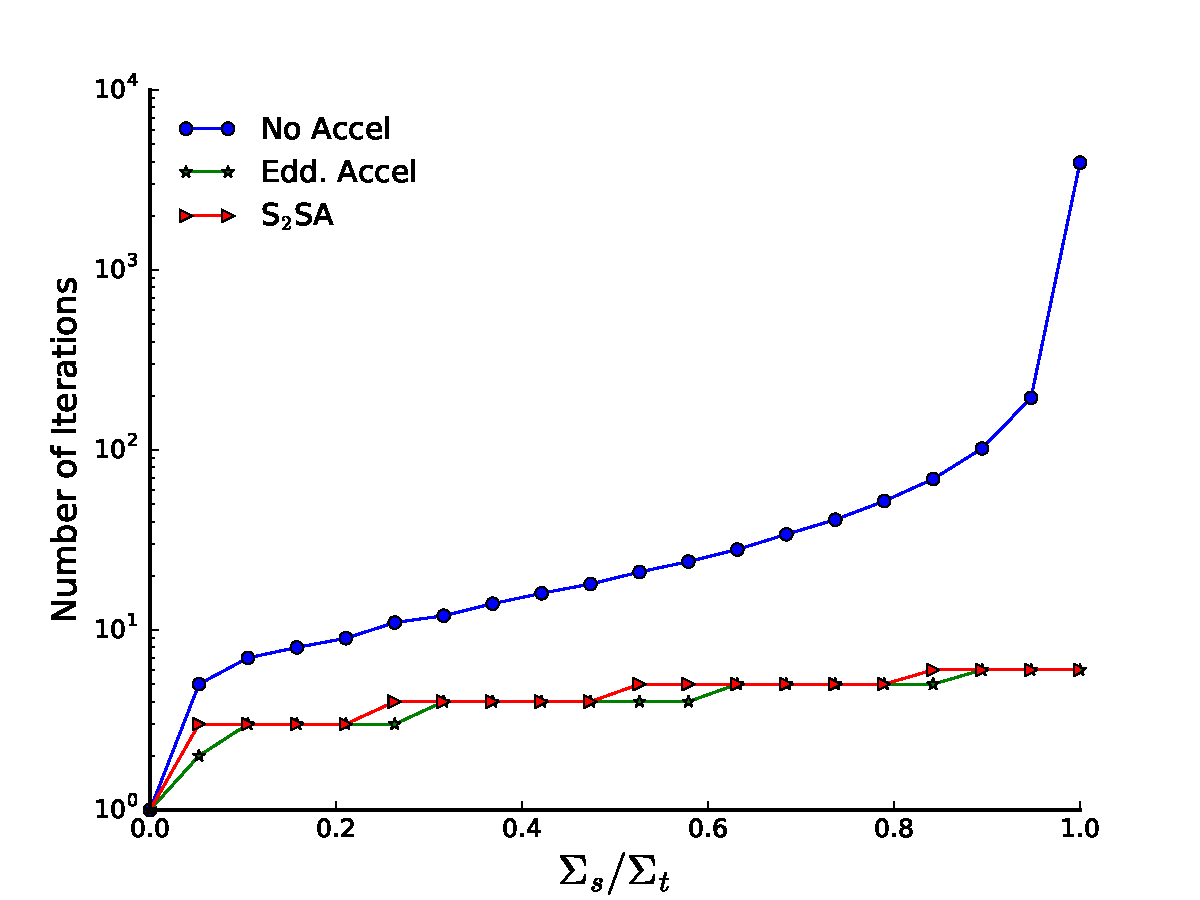
\includegraphics[width=.55\paperwidth]{figs/accel.pdf}}

%     Accelerates between 2.5 and 650 times $\Rightarrow$ acceleration is occurring 

%     Performs similarly to consistent acceleration scheme 

% \end{frame}

\begin{frame}{Diffusion Limit}

	\footnotesize
	\onslide<+->
	Scale cross sections, source 
	$$\Sigma_t \rightarrow \Sigma_t/\epsilon $$
	$$\Sigma_a \rightarrow \epsilon \Sigma_a$$
	$$Q \rightarrow \epsilon Q$$ 

	System becomes diffusive as $\epsilon \rightarrow 0$ 

	\onslide<+->
	\centerline{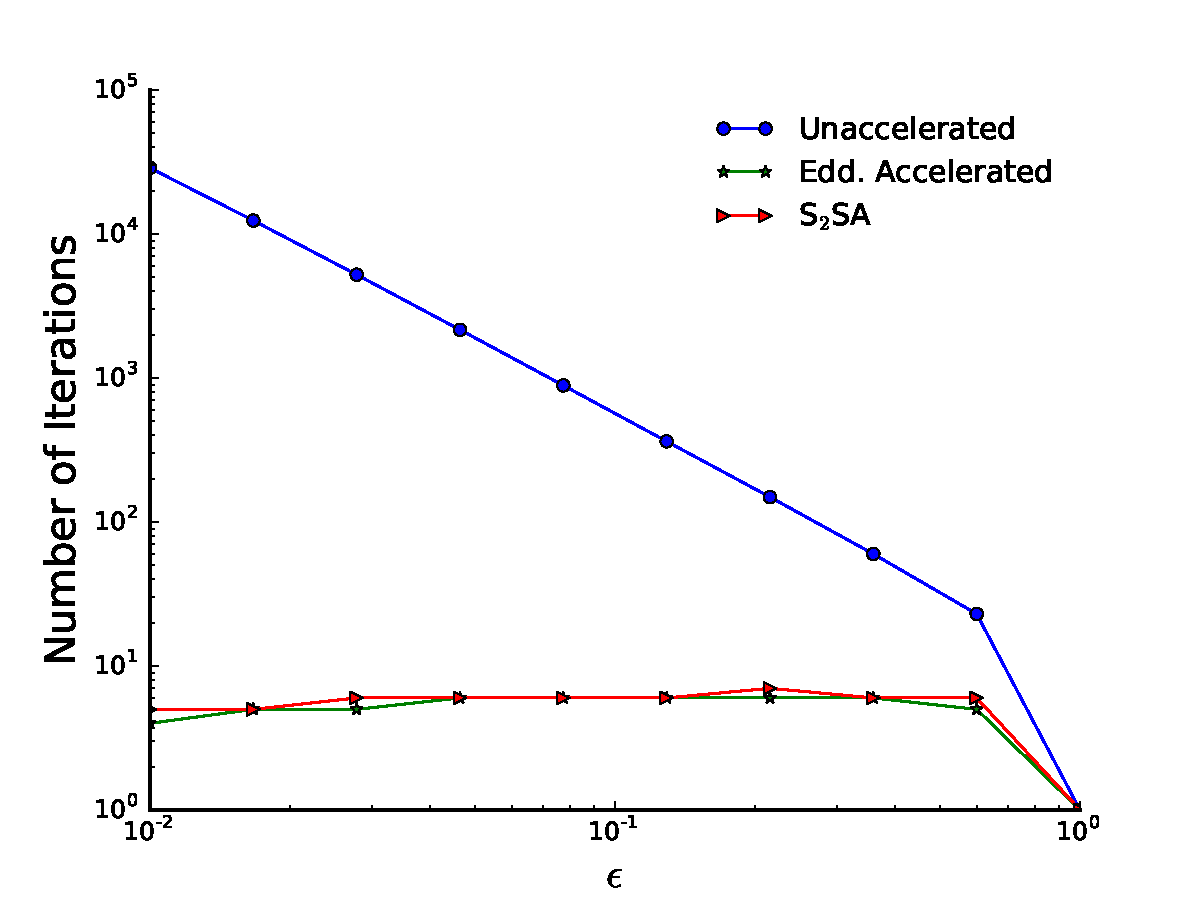
\includegraphics[width=.5\paperwidth]{figs/diffLimit.pdf}}

	\onslide<+->
	Accelerates source iteration, survives diffusion limit 

	\onslide<+->
	Performs similarly to consistently differenced, linear acceleration (S$_2$SA)

\end{frame}

\begin{frame}{Convergence Rate Comparison}

    \onslide<+->
    \begin{columns}
    \begin{column}{.5\paperwidth}
    \begin{figure} \centering
    	Unaccelerated
        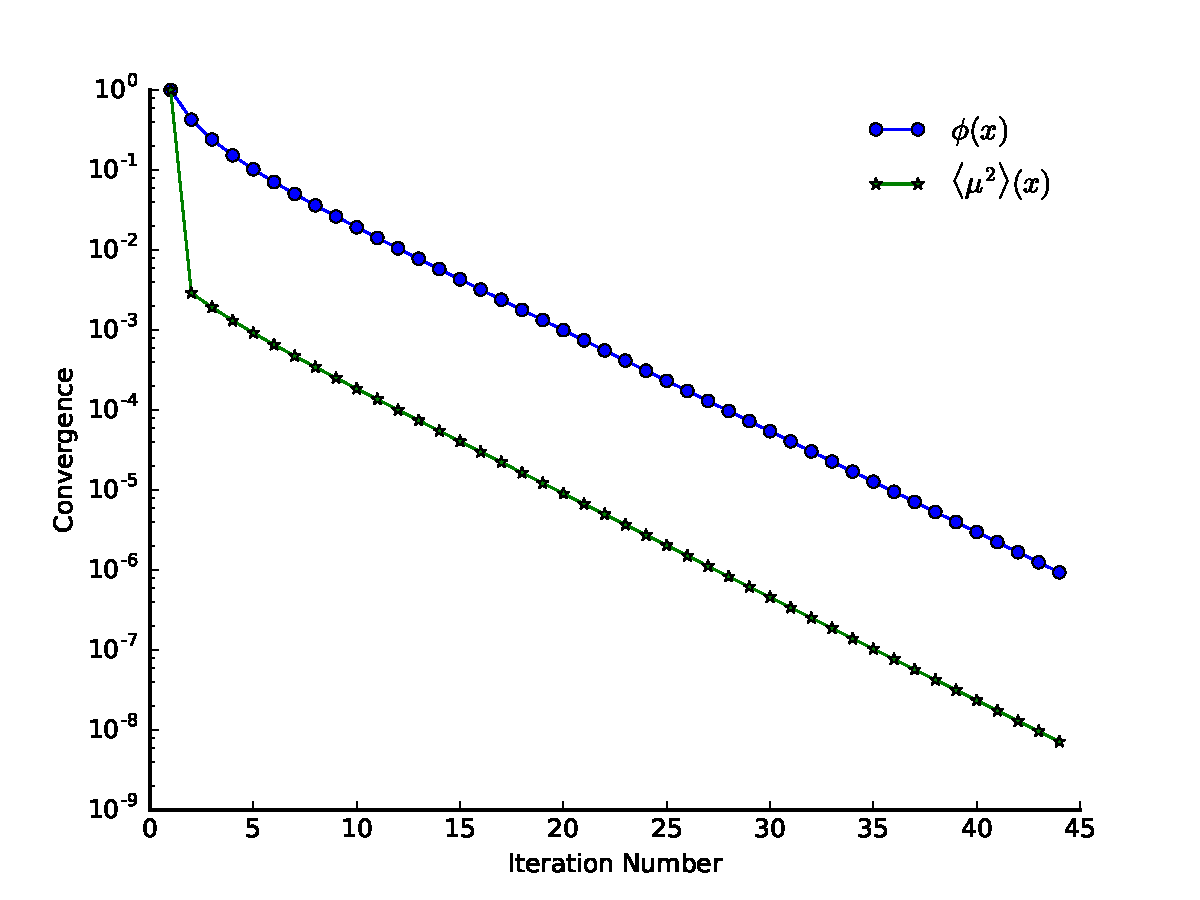
\includegraphics[width=.45\paperwidth]{figs/converge_una.pdf}
    \end{figure}
    \end{column}
    \begin{column}{.5\paperwidth}
    \begin{figure} \centering
    	Accelerated
        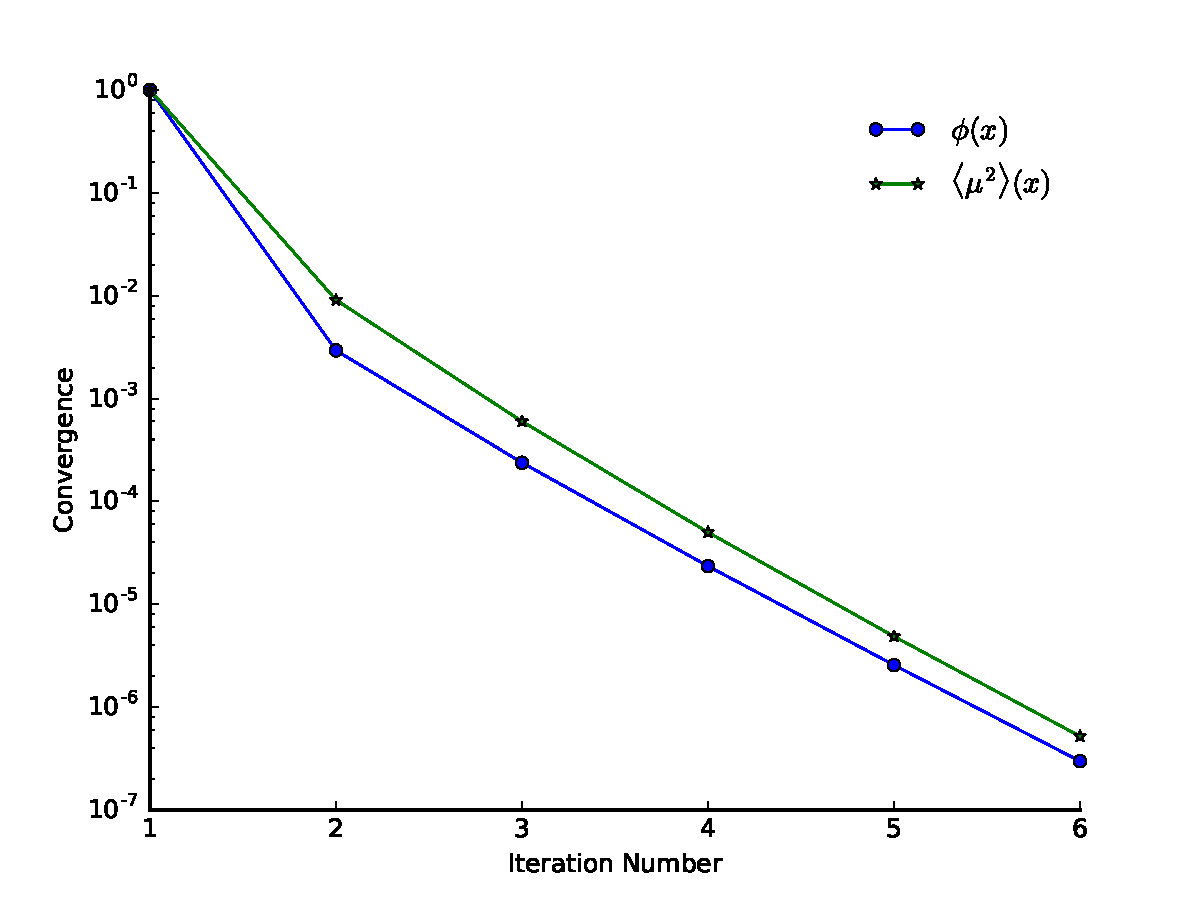
\includegraphics[width=.45\paperwidth]{figs/converge_acc.pdf}
    \end{figure}
   	\end{column}
   	\end{columns}

    \onslide<+->
    \vfill
    \centerline{\textbf{Fast rate of convergence of $\edd(x)$ is transfered to $\phi(x)$}}

\end{frame}

\begin{frame}{Solution Convergence}

	\onslide<+->
	Compare 
	\begin{equation*}
		\frac{\| \phi_{\text{S}_N}(x) - 
			\phi_\text{Moment}(x)\|}{\|\phi_\text{Moment}(x) \|}
	\end{equation*}
	as $h\rightarrow 0$ 

	\onslide<+->
	\centerline{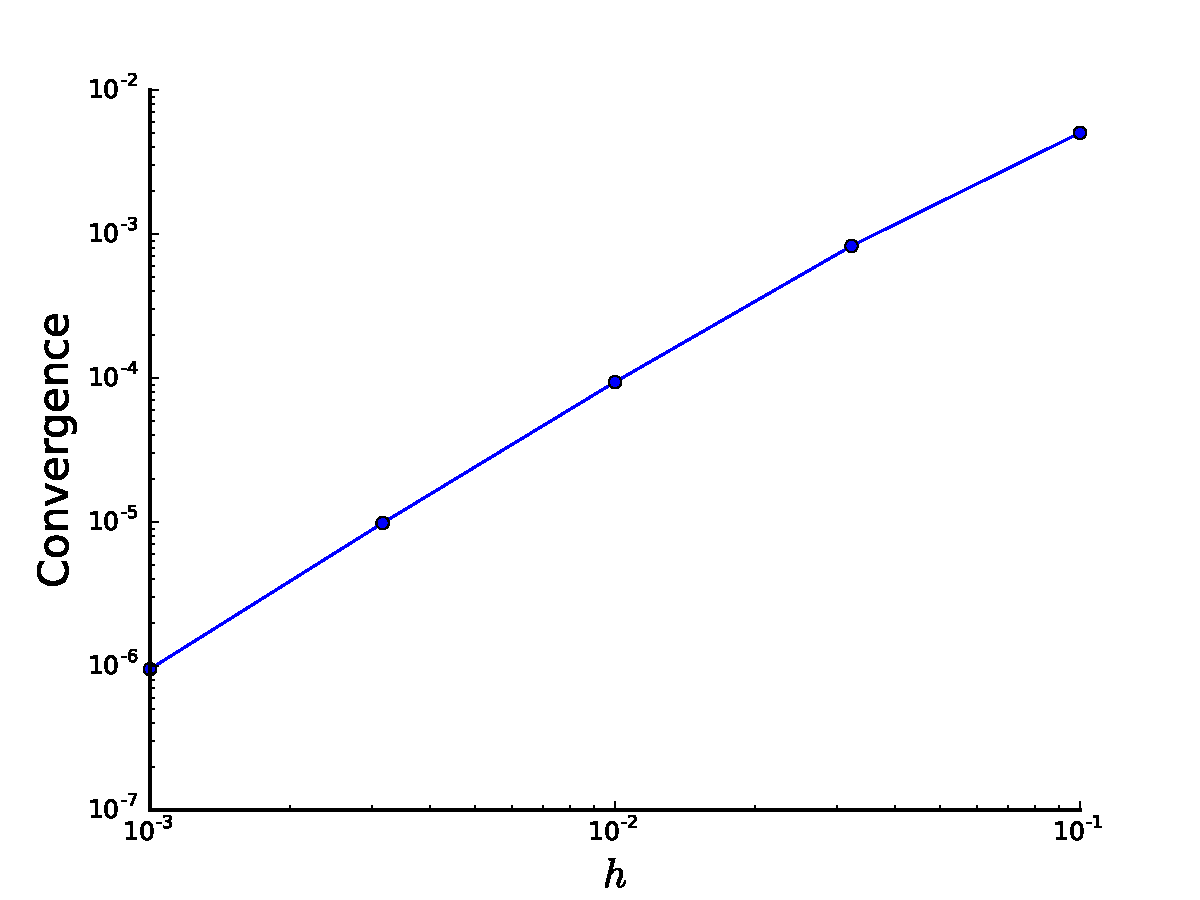
\includegraphics[width=.5\paperwidth]{figs/hlim.pdf}}

	\onslide<+->
	\SN and Moment solutions converge as mesh is refined 

\end{frame}

\begin{frame}{Method of Manufactured Solutions Order of Accuracy} 

	Set source term to force solution to 
	\begin{equation*}
		\phi(x) = \sin\left(\frac{\pi x}{x_b}\right)
	\end{equation*}

	\pause
	\centerline{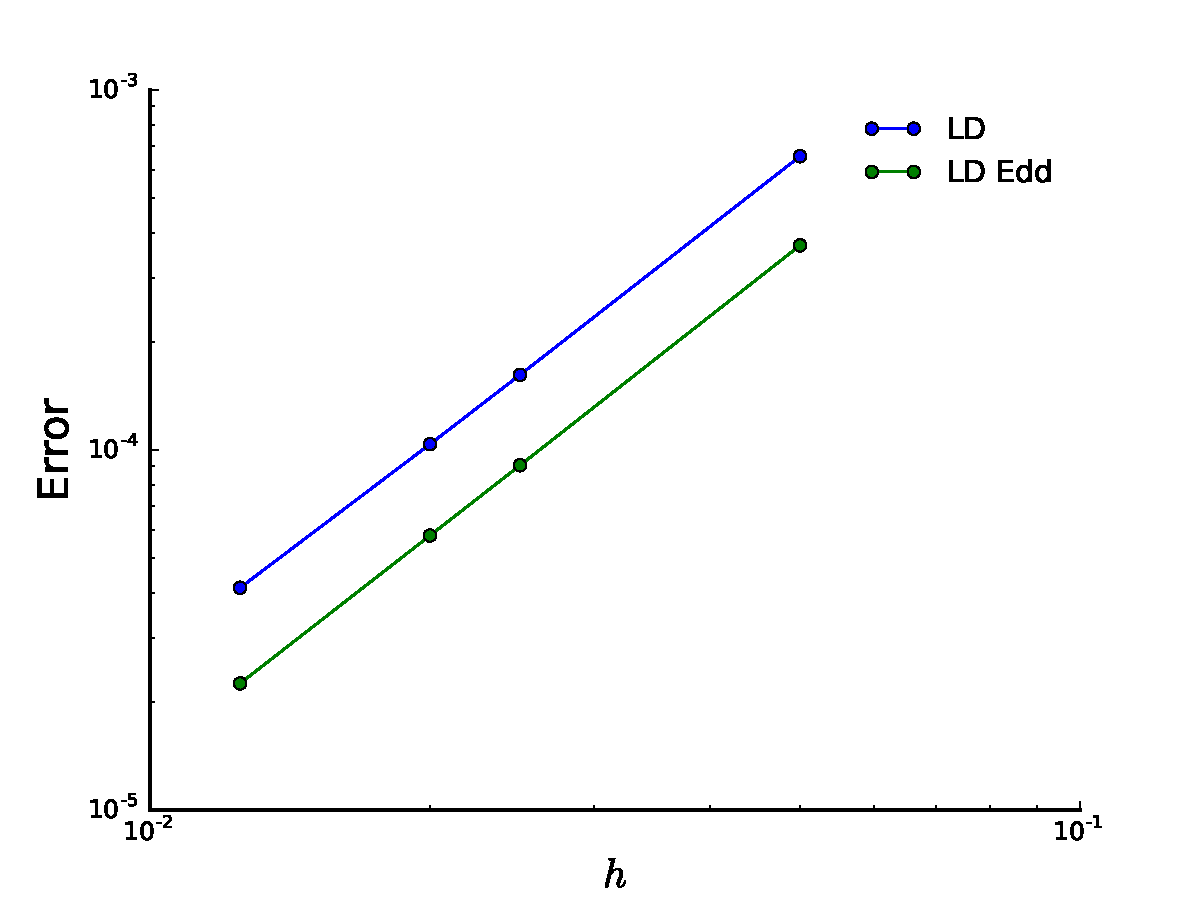
\includegraphics[width=.5\paperwidth]{figs/ooa.pdf}}

	\pause
	Both second order accurate

	\pause
	Eddington Acceleration did not effect the order of accuracy of lumped LDG 

\end{frame}

\section{Conclusions}

\begin{frame}{Summary}

    \onslide<+->
    Conclusions
    \begin{itemize} \vspace{-.1in}
        \item Scheme successfully accelerated source iteration in 1D slab geometry 

        % \item Inherently compatible with rad-hydro multiphysics 

        % \begin{itemize}
        %     \item Transport and acceleration steps can be discretized with arbitrarily different methods 
        %     \item Avoids consistency issues 
        %     \item Provides less expensive, conservative solution 
        % \end{itemize}

        \item Eddington Acceleration is uniquely suited for radiation hydrodynamics 
        \begin{itemize}
        	\item LDG transport 
        	\item MHFEM hydrodynamics 
        	\item Source iteration acceleration 
        	\item Provides inexpensive, conservative solution 
        \end{itemize}

        \item Proved MHFEM can be used to accelerate lumped LDG transport in 1D slab geometry 

    \end{itemize}

    \onslide<+->
    Future Work 
    \begin{itemize} \vspace{-.1in}
        \item Develop a rad-hydro algorithm 

        \begin{itemize}
            \item Make use of inexpensive Moment solution in multiphysics iterations 
        \end{itemize}

        \item Add energy, time dependence 

        \item Test in 3D 

        % \item P$_N$ scattering/source expansion  

        \item Explore other multiphysics applications 

    \end{itemize}

\end{frame}

% begin uncounted slides ---------------------------
\appendix

\begin{frame}{References}

    \nocite{adams,morel,llnl,alcouffe,mhfem,hydro,bolding}
    \setbeamerfont{bibliography item}{size=\footnotesize}
    \setbeamerfont{bibliography entry author}{size=\footnotesize}
    \setbeamerfont{bibliography entry title}{size=\footnotesize}
    \setbeamerfont{bibliography entry location}{size=\footnotesize}
    \setbeamerfont{bibliography entry note}{size=\footnotesize}
    \setbeamertemplate{bibliography item}{\insertbiblabel}
    \bibliographystyle{siam}
    \bibliography{bibliography}

\end{frame}

\begin{frame}[standout]
  Questions?
\end{frame}

\begin{frame}{S$_8$ v. Diffusion}

    Small system $\Rightarrow$ diffusion not expected to be accurate 
    \begin{center}
    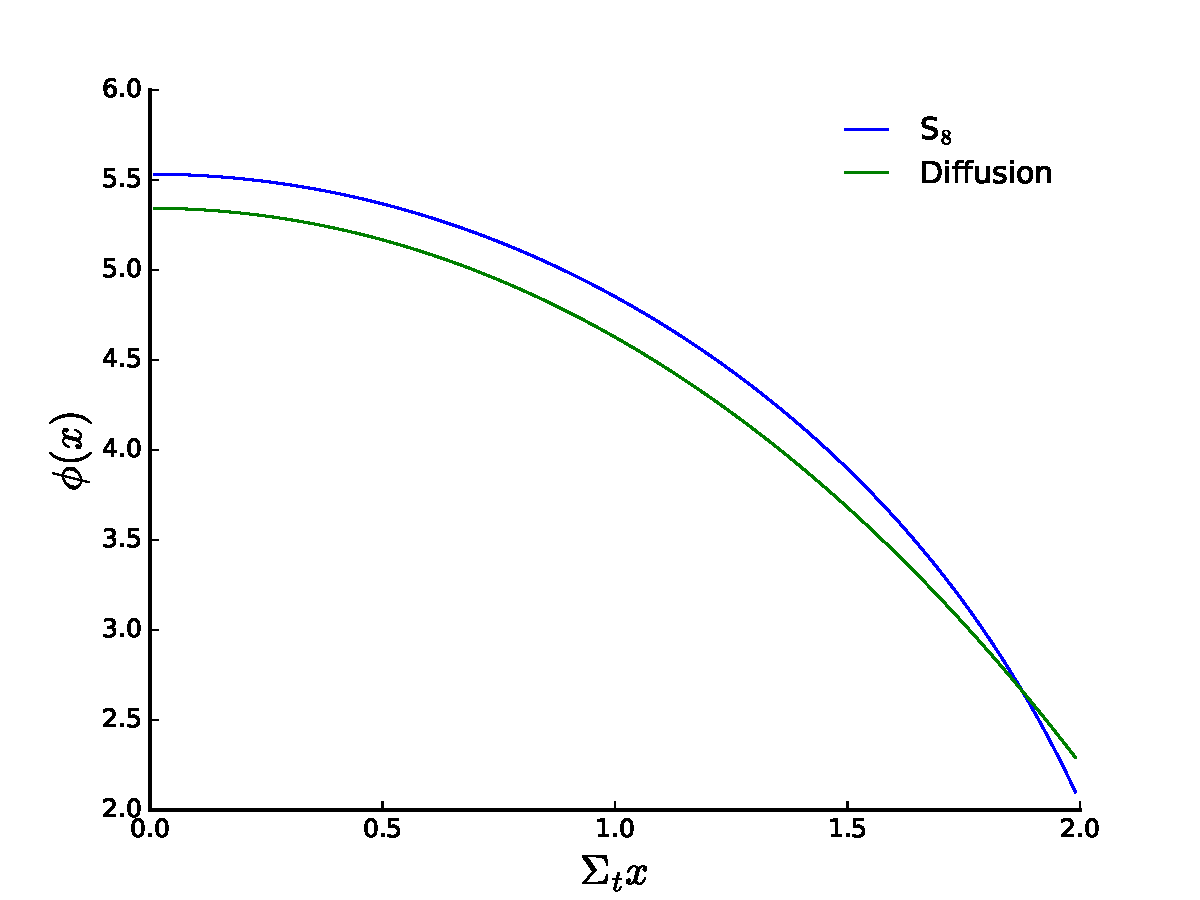
\includegraphics[width=.45\paperwidth]{figs/dvs.pdf}
    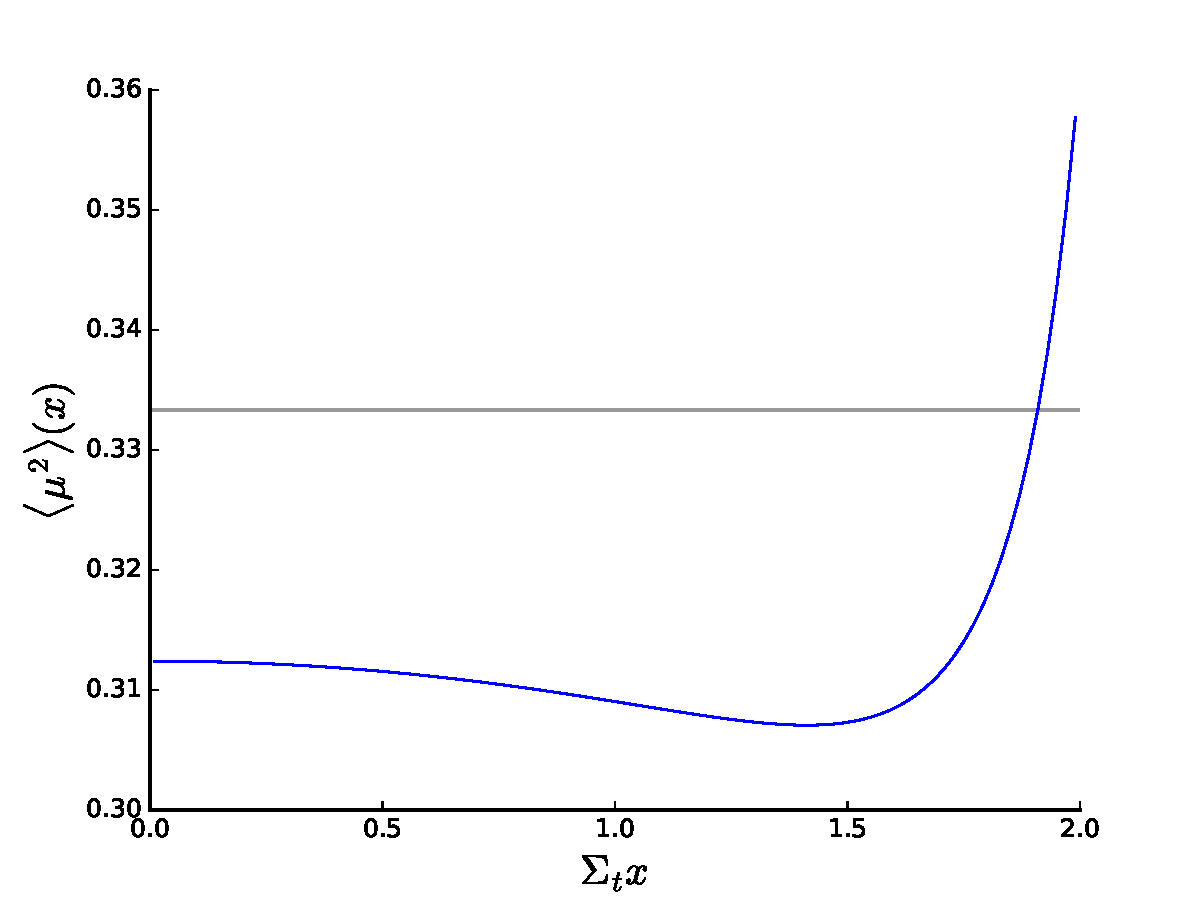
\includegraphics[width=.45\paperwidth]{figs/edd.pdf}
    \end{center}

\end{frame}

\begin{frame}{S$_8$ v. Drift Diffusion}

    \onslide<+->
    Use $\edd(x)$ from S$_8$ in Moment Equations
    \begin{center}
    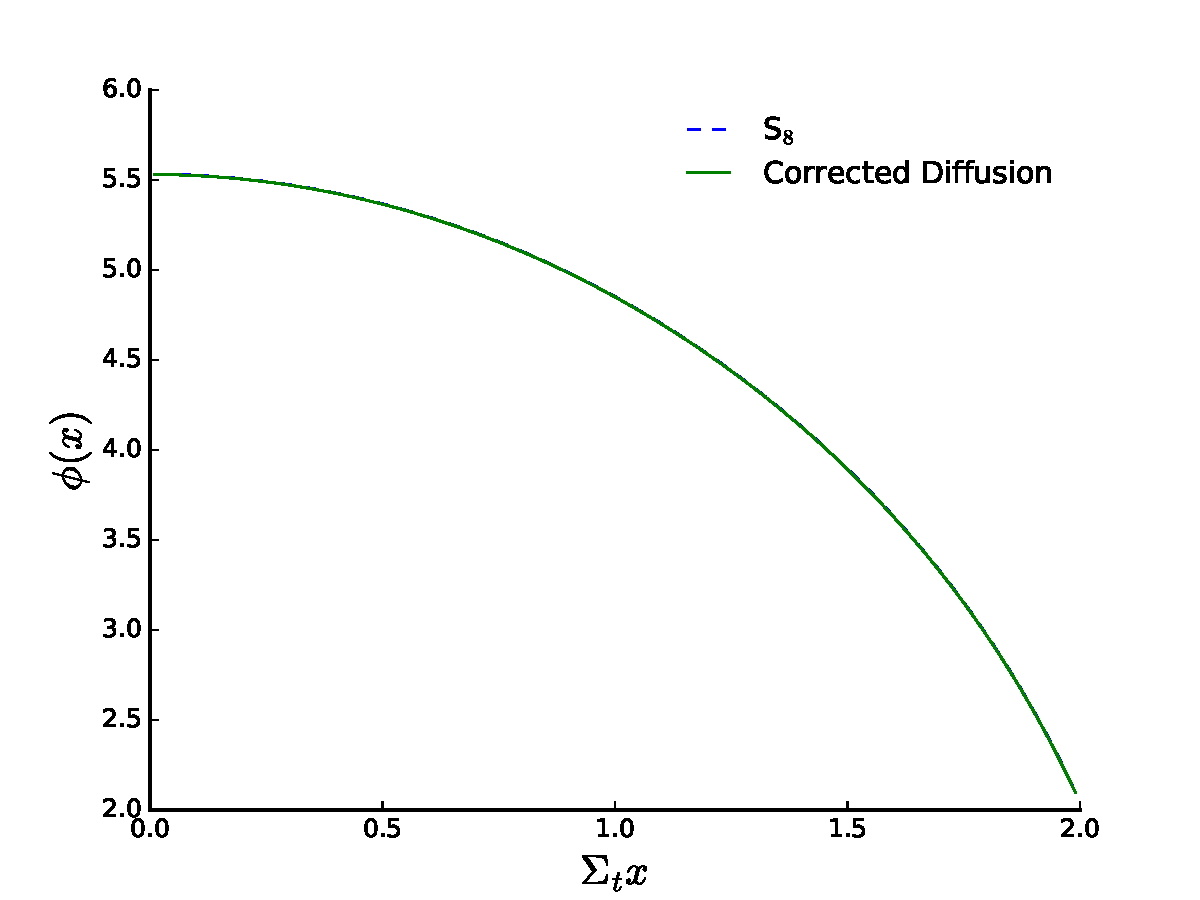
\includegraphics[width=.5\paperwidth]{figs/corrected.pdf}
    \end{center}

    \onslide<+->
    Moment Equations and \SN match! 

    \onslide<+-> 
    Requires knowledge of angular flux

\end{frame}

\end{document}
